%!TEX encoding = UTF-8 Unicode
\documentclass[ % options,
    a4paper,    % papersize
%    cjk,       % for cjk-ko
%    usedotemph,% for cjk-ko's \dotemph
    amsmath,    % load amsmath.sty to typeset math materials
    itemph,     % to disable gremph default (xe/lua)
%    footnote,  % korean style footnote
%    chapter,   % to use \chapter
]{oblivoir}     % xoblivoir and oblivoir are identical.

\ifPDFTeX       % latex, pdflatex
%    \usepackage{newtxtext}    % Latin fonts
\else\ifLuaOrXeTeX   % xelatex or lualatex
%  \setmainfont{TeX Gyre Termes}   %% Latin fonts
%	\setkomainfont(Noto Serif CJK KR)(* Bold)(* Medium)
%	\setkosansfont(Noto Sans CJK KR)(* Bold)(* Medium)
\fi\fi

% color 
\usepackage{xcolor}
\usepackage{titlesec}
\titleformat{\section}{\color{blue}\normalfont\Large\bfseries}{\color{blue}\thesection}{1em}{}
\titleformat{\subsection}{\color{orange}\normalfont\Large\bfseries}{\color{orange}\thesubsection}{1em}{}

% packages
\usepackage{kotex-logo}
\usepackage[utf]{kotex}
\usepackage{geometry}
 \geometry{
 a4paper,
 total={170mm,257mm},
 left=20mm,
 top=20mm,
 }
 
%% font packages and setup
\usepackage{fontspec}
\setmainfont{UnDotum}
\setsansfont{UnDotum}
\setmonofont{UnTaza}
\usepackage{dhucs-interword}
\interhword[.6]{.475}{.1}{.1}
\setlength{\parindent}{0em}
\setlength{\parskip}{1em}

% operator
\DeclareMathOperator*{\argmax}{argmax}
\DeclareMathOperator{\E}{\mathbb{E}}

% image 
\usepackage{graphicx}

% page header
\usepackage{fancyhdr}
\pagestyle{fancy}
\rhead{강화학습}

% box 
\usepackage{tcolorbox}

% 정의와 정리 등
\usepackage{amsthm}


\theoremstyle{theorem}
\newtheorem{theorem}{Theorem}

\theoremstyle{theorem}
\newtheorem{proposition}{Proposition}[theorem]

\theoremstyle{theorem}
\newtheorem{lemma}{Lemma}[theorem]

\theoremstyle{definition}
\newtheorem{definition}{Definition}[theorem]

\theoremstyle{remark}
\newtheorem*{remark}{Remark}


\begin{document}

\title{Policy Gradient Algorithms}
\author{wisemountain}
\date{\today}

\maketitle

\newpage

\tableofcontents

\newpage

\section{개요}

RL의 기본 알고리즘을 살사와 큐 러닝을 중심으로 이해하고 나서 앞으로 나아가려고 하면 
정책 기반의 알고리즘을 만나게 된다. 이 때 잘 이해가 안 되는 여러 용어들과 
좀 더 깊은 이해가 필요한 다양한 영역을 만나게 된다. 

그 첫 관문으로 정책 경사 정리 (Policy Gradient Theorem)가 있다. 

\begin{center}
\includegraphics{2_pgt}
\end{center}

https://lilianweng.github.io/lil-log/2018/04/08/policy-gradient-algorithms.html

openai의 엔지니어가 잘 정리해 놓은 사이트이고 여기에 모든 정책경사(Policy Gradient) 기반 
알로그즘이 대부분 있다. 

이 문서의 목표는 여기에 있는 내용들을 이해하는 것이다. 

\section{PGT의 증명}

\subsection{MCMC의 이해}

https://jeremykun.com/2015/04/06/markov-chain-monte-carlo-without-all-the-bullshit/

PGT에서 사용하는 정상 상태 $d^\pi(s)$ 를 이해하려면 MCMC를 MDP 보다 약간 더 이해해야 한다. 

\begin{tcolorbox}
The problem is drawing from a distribution
\end{tcolorbox}

MCMC는 복잡한 분포에서 효율적으로 샘플링을 하는 방법에 관한 것이다. 

문서에서는 아이의 이름으로 쓰일 확률을 알려주는 마법의 상자를 가정한다. 
그리고, 이름 별로 부여된 확률은 변하지 않는다. 

\begin{definition}[the sampling problem]
Let $D$ be a distribution over a finite set $X$. Give p.d.f $p(x)$, 
design an efficient randomized algorithm $A$ which outputs an element of $X$, 
so that the probability of outputting $x$ is approximately $p(x)$. 
More generally, output a sample of elements from $X$ drawn according 
to $p(x)$.

\end{definition}

위는 확률 분포 D를 갖는 유한집합 X에 대해 확률밀도함수 p(x)를 알 수 있을 때, 
어떻게 샘플링을 해야 원래 X의 분포 D에 근접하게 뽑아낼 수 있을 지를 찾는 
알고리즘이 MCMC라고 말하고자 한다. 그러니까 그냥 몬테 카를로 방법을 
좀 분포를 알기 어려운 집합에 적용하는 똑똑한 방법이라 할 수 있다. 

\begin{tcolorbox}
Random Walks, the "Markov Chain" part of MCMC
\end{tcolorbox}

마르코프 체인은 그래프 상의 랜덤워크를 멋지게 부르는 이름일 뿐이다. 

여기서 마르코프 체인은 마르코프 프로세스와 같은 의미이고, 이는 
강화학습을 살펴볼 때 마르코프 성질을 갖는 확률 과정 (상태 그래프 상의 랜덤워크) 
이라는 걸 알았다. 

여기서는 상태 전환이 아닌 그래프로 설명하고 있다. 그래프로 보면 
좀 더 공간에 배치된 기하를 떠올리게 되므로 생생해지는 효과가 있다. 

\begin{center}
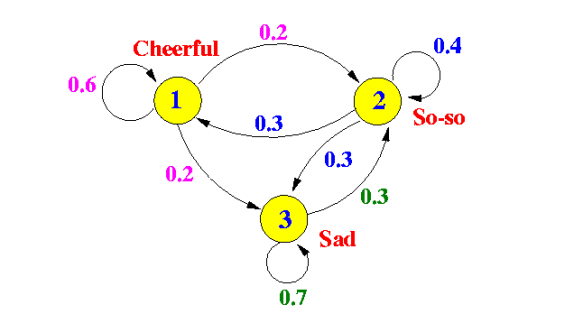
\includegraphics[scale=0.5]{3_markov_chain}
\end{center}

그림에서 0.2, 0.3 등이 다음 꼭지점으로 갈 확률이고 상태 전환 확률로 
생각하면 된다. 한 꼭지점에서 나가는 확률의 합은 1이 되어야 한다. 

정상분포 정리(statinary distribution theorem)은 마르코프 체인의 근본정리로도 
불린다. 이걸 이해하는 것이 이 문서를 읽는 목적이다. 

정상분포란 확률 그래프의 랜덤워크를 아주 오래 했을 때 특정 꼭지점(상태)에 
있게 될 확률이다. 

하지만 모든 마르코프 체인이 정상분포를 갖지는 않고, 필요한 조건이 
그래프 $G$가 강하게 연결되어 있어야 한다. 그래프가 연결되어 있다는 뜻은 
모든 꼭지점에서 모든 꼭지점으로 변(edge)을 따라 갈 수 있는 경로가 있다는 뜻이고, 
강하게 연결되어 있다는 뜻은 이동 방향을 고려할 때도 연결되어 있다는 뜻이다. 

강한 연결과 다음의 정리는 동치이다. 

\begin{theorem}
모든 $v \in G$에 대해, $v$에서 시작한 무한한 랜덤워크는 $v$로 확률 1로 
다시 올 수 있다. 또는 $v$로 되돌아 오는 무한한 랜덤워크가 있다. 
\end{theorem}

이렇게 보면 대체로 강한연결은 대부분의 랜덤워크에서 가능해 보이고, 
필요하면 그렇게 되도록 "설계"할 수 있어 보인다. 

좀 더 익숙한 선형대수를 사용하여 정상분포를 설명하기 위해 
전이행렬 $A = (a_{i, j})$, $a_{i,j} = p_{(i, j)}$로 둔다. 

이와 같이 전이행렬을 구성하고, 기저 벡터(basis vector) $e_i$를 
$i$번째 정점(꼭지점)에 있는 상태로 하면, $Ae_i$의 $j$번째 값은 
$j$번째 정점으로 전이할 확률이 된다. 

이와 비슷하게 각 정점에 있을 확률 $q$를 주면 $Aq$는 다음에 
전이할 각 꼭지점에 대한 확률이 된다. 

정상분포 $\pi$는 $A\pi= \pi$가 되는 그러한 $\pi$이고 
이는 $A$의 고유값(eigen value)이 1인 고유벡터(eigen vector)이다. 

\begin{theorem}
G가 강한연결 그래프이고, 각 변의 전이확률이 $\{p_e\}_{e \in E}$ 이고, 
확률 벡터 $x_0$, $x_{t+1} = Ax_t, t \ge 1$, $v_t = \frac{1}{t}\sum_{s=1}^t x_s$로 
주어졌을 때, 다음이 성립한다. 
\begin{enumerate}
\item $\exists \pi . A\pi = \pi$
\item $\forall x_0 . \lim_{t \to \infty} v_t = \pi$

\end{enumerate}

\end{theorem}

증명은 $|Av_t - v_t| \to 0|$을 보이고, 페론-프로베니우스 (Perron-Frobenius) 정리를 참조하여 
고유벡터의 존재를 보장한다는 걸 확인한다. 페론-프로베니우스의 정리의 이해는 아직 준비가 덜 되어 
위의 정리를 그냥 인정하고 진행한다. 

\begin{tcolorbox}
Constructing a graph to walk on
\end{tcolorbox}

원래 MCMC의 목표인 $X$의 분포 $p(x)$를 잘 보여주는 샘플링 알고리즘을 만든다는 것으로 
다시 돌아온다. MCMC 알고리즘은 마르코프 체인을 잘 구성해서 분포를 모름에도 
정상분포가 $p(x)$가 되도록 하는 것이다. 

이제 정상분포로 수렴하는 적절하면서 빠르게 수렴하는 좋은 그래프를 찾으면 된다. 
빠르게 수렴하는 그래프는 해당 블로그 포스팅의 설명 범위를 넘어선다고 한다. 

이런 그래프를 찾는 알고리즘 중 Metropolis-Hastings 알고리즘을 선택한다. 
입력은 $p(x)$이고, 출력은 정점이 $X$인 그래프 상의 랜덤워크를 구성하는 규칙이다. 

래티스를 사용하고 전이하는 확률 규칙을 지정하여 


\end{document}
























